\section{Векторы. Линейная зависимость системы векторов. Базис линейного пространства. Скалярное произведение векторов.}

\textbf{Вектор} — это направленный отрезок, который характеризует величину и направление. Геометрически его можно представить как стрелку от начала координат до некоторой точки.

Алгебраически вектор в $n$-мерном пространстве $\mathbb{R}^n$ — это упорядоченный набор чисел:
\[
\vec{v} = (v_1, v_2, \dots, v_n)
\]

\textbf{Примеры:}
\[
\vec{a} = (3, -1), \quad \vec{b} = (1, 2, 4)
\]

\vspace{1em}
\textbf{Геометрическая интерпретация:}
\begin{center}
\begin{tikzpicture}[scale=1.2,>=stealth]
\draw[->,gray!40] (-1,0) -- (4,0) node[right] {$x$};
\draw[->,gray!40] (0,-1) -- (0,3) node[above] {$y$};
\draw[->,blue,thick] (0,0) -- (2.5,1.5) node[above right] {$\vec{v}$};
\end{tikzpicture}
\end{center}

\vspace{1em}
\textbf{Основные операции:}
\begin{itemize}
  \item \textbf{Сложение:} $(x_1, y_1) + (x_2, y_2) = (x_1 + x_2, y_1 + y_2)$
  \item \textbf{Умножение на скаляр:} $\lambda \cdot (x, y) = (\lambda x, \lambda y)$
  \item \textbf{Нулевой вектор:} $\vec{0} = (0, 0, \dots, 0)$
\end{itemize}

\begin{center}
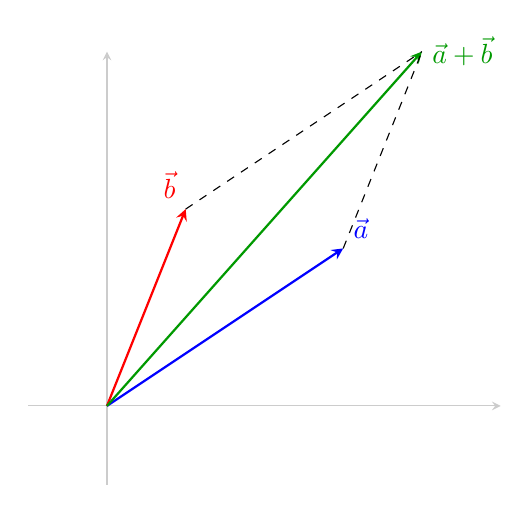
\begin{tikzpicture}[scale=1.0,>=stealth]
\draw[->,gray!40] (-1,0) -- (5,0);
\draw[->,gray!40] (0,-1) -- (0,4.5);

\draw[->,blue,thick] (0,0) -- (3,2) node[above right] {$\vec{a}$};
\draw[->,red,thick] (0,0) -- (1,2.5) node[above left] {$\vec{b}$};
\draw[->,green!60!black,thick] (0,0) -- (4,4.5) node[right] {$\vec{a} + \vec{b}$};

\draw[dashed] (3,2) -- (4,4.5);
\draw[dashed] (1,2.5) -- (4,4.5);
\end{tikzpicture}
\end{center}

\vspace{2em}
\textbf{Линейная зависимость и независимость векторов:}

Рассмотрим векторы $\vec{v}_1, \vec{v}_2, \dots, \vec{v}_k$. Если существует набор коэффициентов $\lambda_1, \dots, \lambda_k$ (не все нули), такой что:
\[
\lambda_1 \vec{v}_1 + \dots + \lambda_k \vec{v}_k = \vec{0}
\]
то векторы — \textbf{линейно зависимы}.

Если единственное решение — тривиальное ($\lambda_1 = \dots = \lambda_k = 0$), то векторы — \textbf{линейно независимы}.

\textbf{Пример:}
\[
\vec{v}_1 = (1, 2), \quad \vec{v}_2 = (2, 4) \Rightarrow \vec{v}_2 = 2 \vec{v}_1 \Rightarrow \text{зависимы}
\]

\begin{center}
\begin{tikzpicture}[scale=1.2,>=stealth]
\draw[->,gray!40] (-0.5,0) -- (3,0);
\draw[->,gray!40] (0,-0.5) -- (0,3);
\draw[->,blue,thick] (0,0) -- (1,2) node[above left] {$\vec{v}_1$};
\draw[->,red,thick] (0,0) -- (2,4) node[above right] {$\vec{v}_2$};
\end{tikzpicture}
\end{center}

\vspace{2em}
\textbf{Базис линейного пространства:}

Базис — это система линейно независимых векторов, которая порождает всё пространство.  
Любой вектор пространства выражается через базис как линейная комбинация.

В $\mathbb{R}^2$ стандартный базис:
\[
\vec{e}_1 = (1, 0), \quad \vec{e}_2 = (0, 1)
\Rightarrow \vec{v} = x \vec{e}_1 + y \vec{e}_2
\]

\begin{center}
\begin{tikzpicture}[scale=1.1,>=stealth]
\draw[->,gray!40] (-0.5,0) -- (3.5,0) node[right] {$x$};
\draw[->,gray!40] (0,-0.5) -- (0,3.5) node[above] {$y$};

\draw[->,thick] (0,0) -- (2,0) node[below] {$x\vec{e}_1$};
\draw[->,thick] (2,0) -- (2,1.5) node[right] {$y\vec{e}_2$};
\draw[->,blue,thick] (0,0) -- (2,1.5) node[above right] {$\vec{v}$};
\end{tikzpicture}
\end{center}

Размерность пространства — это количество векторов в базисе. Например, в $\mathbb{R}^3$ базис содержит 3 вектора.

\vspace{2em}
\textbf{Скалярное произведение векторов:}

Скалярное произведение двух векторов $\vec{a} = (a_1, \dots, a_n)$ и $\vec{b} = (b_1, \dots, b_n)$:
\[
\langle \vec{a}, \vec{b} \rangle = a_1 b_1 + a_2 b_2 + \dots + a_n b_n
\]

\textbf{Пример:}
\[
\vec{a} = (1, 2), \quad \vec{b} = (3, 4) \Rightarrow \langle \vec{a}, \vec{b} \rangle = 1\cdot3 + 2\cdot4 = 11
\]

\textbf{Свойства:}
\begin{itemize}
  \item Симметрия: $\langle \vec{a}, \vec{b} \rangle = \langle \vec{b}, \vec{a} \rangle$
  \item Линейность: $\langle \alpha \vec{a} + \beta \vec{c}, \vec{b} \rangle = \alpha \langle \vec{a}, \vec{b} \rangle + \beta \langle \vec{c}, \vec{b} \rangle$
  \item $\langle \vec{a}, \vec{a} \rangle = \|\vec{a}\|^2$
\end{itemize}

\textbf{Геометрически:}
\[
\langle \vec{a}, \vec{b} \rangle = \|\vec{a}\|\|\vec{b}\|\cos\theta
\]
где $\theta$ — угол между векторами.  
Если $\langle \vec{a}, \vec{b} \rangle = 0$ — векторы ортогональны (перпендикулярны).

\begin{center}
\begin{tikzpicture}[scale=1.2,>=stealth]
\coordinate (O) at (0,0);
\coordinate (A) at (2,0);
\coordinate (B) at (1,2);
\draw[->,gray!40] (-0.5,0) -- (3,0);
\draw[->,gray!40] (0,-0.5) -- (0,3);
\draw[->,thick] (O) -- (A) node[below] {$\vec{a}$};
\draw[->,thick] (O) -- (B) node[above] {$\vec{b}$};
\draw (1,0) arc[start angle=0,end angle=63,radius=1cm];
\node at (1.1,0.2) {$\theta$};
\end{tikzpicture}
\end{center}

\vspace{2em}
\textbf{Длина вектора (норма):}
\[
\|\vec{a}\| = \sqrt{\langle \vec{a}, \vec{a} \rangle}
\]

\textbf{Угол между векторами:}
\[
\cos\theta = \frac{\langle \vec{a}, \vec{b} \rangle}{\|\vec{a}\|\|\vec{b}\|}
\]

---

\textbf{Итоги:}
\begin{itemize}
  \item Векторы — фундаментальные объекты в линейной алгебре.
  \item Линейная зависимость помогает понимать структуру пространства.
  \item Базис — минимальный набор независимых векторов, порождающих всё пространство.
  \item Скалярное произведение связывает векторы с геометрией — углами и длинами.
\end{itemize}
